
The inner-most detector, closest to the beam pipe, is the CMS tracker system, which uses two technologies: silicon pixels and silicon microstrips (photos of each shown in Fig.~\ref{fig:Tracker}). The purpose of the CMS tracking system is to reconstruct the trajectories of electromagnetically charged physics objects close to the interaction point and measure the positions of the primary vertex (PV) of collisions and secondary vertecies of displaced decays (e.g., B hadrons). Owing to its proximity to the primary-interaction point, the CMS tracker is subject to the highest dosage radiation of all the subsystems.

\begin{figure}[H]
    \centering
    \resizebox{1\textwidth}{!}{
    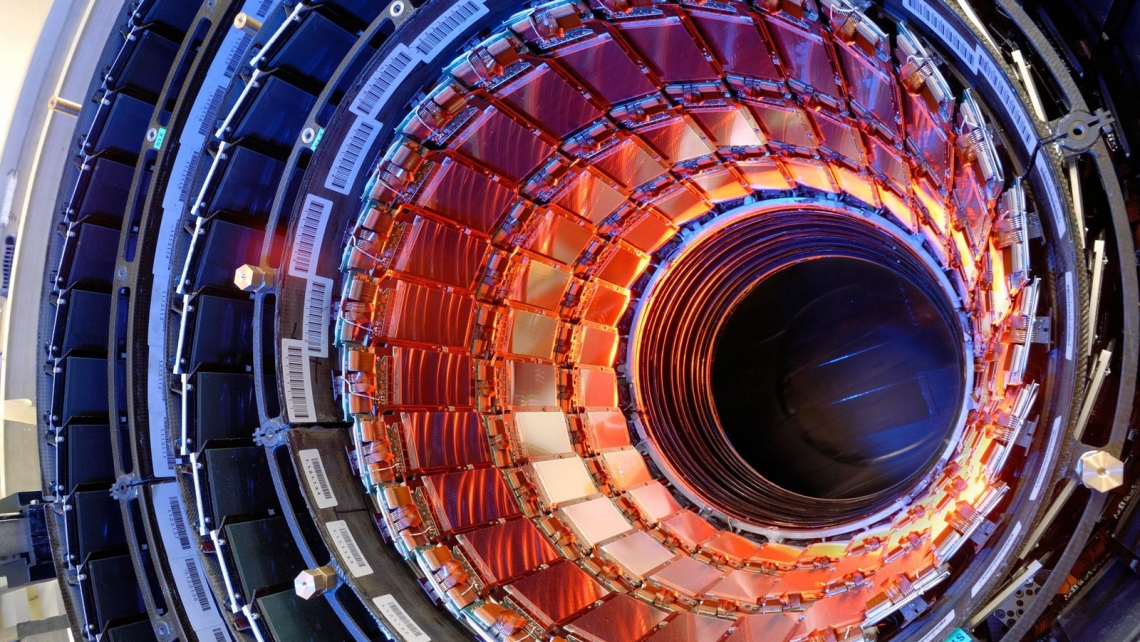
\includegraphics[height=\textwidth]{Images/CMS/SiStripTracker.jpg}
    \quad
    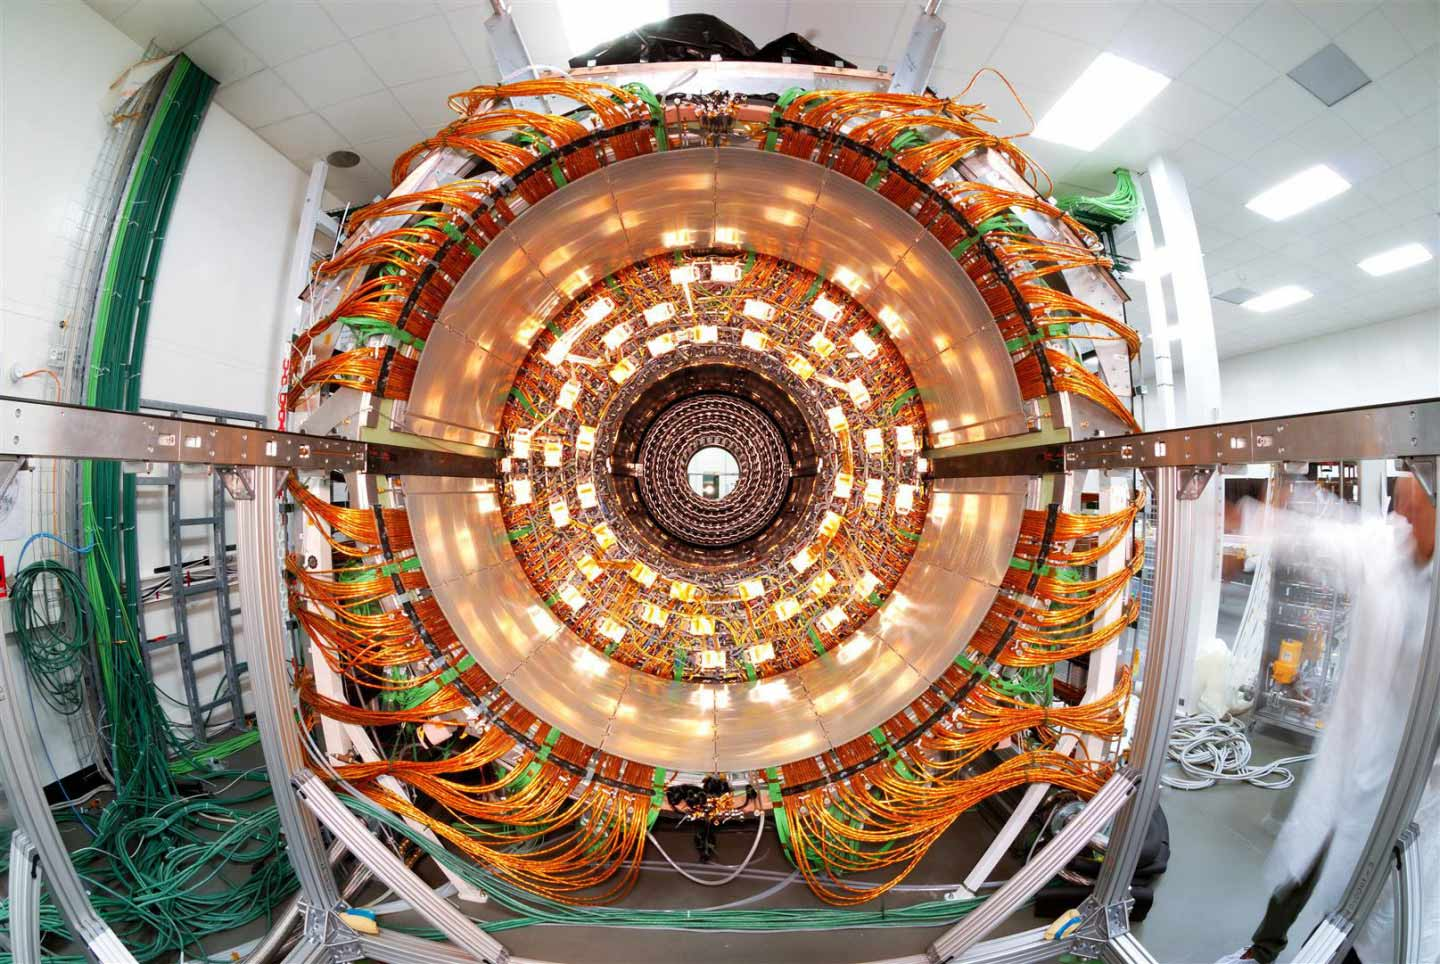
\includegraphics[height=\textwidth]{Images/CMS/PixelTracker.jpg}
    } 
    \caption{Photographs of the silicon strip detectors (left) and the pixel detectors (right) in the tracker barrel prior to installation.}
    \label{fig:Tracker}
\end{figure}

\subsubsection{Pixel tracker} \label{sec:PixelTracker}

The silicon pixel detector, upgraded to the Phase-1 pixel detector \cite{PixelUpgrade} during the 2016-2017 year-end technical stop of Run 2 to cope with higher integrated luminosities, provides a four-hit coverage in the pseudorapidity range $|\eta|<2.5$. This is accomplished through silicon sensor modules, where each module is a $160\times 416$ pixel sensor connected to 16 readout chips. The modules are arranged in two configurations: four concentric barrel pixel detectors (BPIX) with 1,184 modules, and three endcap disk pixel detectors in the forward regions (FPIX) with 672 modules, for a total of 1856 silicon sensor modules and 124 million readout channels. A schematic of the upgraded Phase-1 pixel detector is provided in Fig.~\ref{fig:PixelDiagram} showing the pseudorapidity coverage.

\begin{figure}[H]
    \centering
    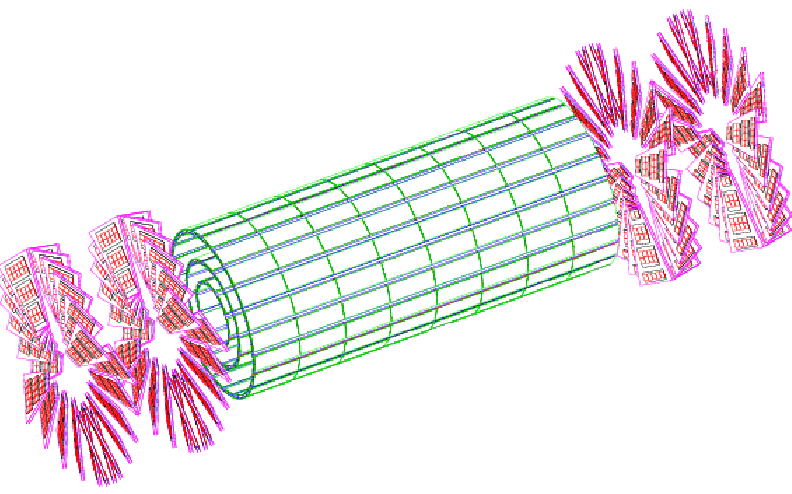
\includegraphics[width=\textwidth]{Images/CMS/PixelDiagram2.png}
    \caption{A diagram of the Phase-1 pixel detector with the BPIX drawn in green and the FPIX drawn in magenta.}
    \label{fig:PixelDiagram}
\end{figure}

\subsubsection{Strip tracker} \label{sec:StripTracker}

Surrounding the pixel detector is the silicon strip tracker \cite{SiliconStrip} which serves the same function as the pixel tracker and covers hits in the same pseudorapidity $|\eta|<2.5$ range. The silicon strip detector is also built with a modular structure, with 15,148 tracker modules each housing one or two silicon sensors totaling 24,244 strip sensors. The silicon strip tracker is divided into four sections: inner barrel (TIB), outer barrel (TOB), inner disks (TID), and outer endcaps (TEC). The TIB and TOB consist of four and six concentric shells respectively, while the TID consists of three disks in each of the forward regions, divided into three concentric rings, and the TEC consists of nine disks with four to seven concentric rings, also in the forward regions. A schematic of the silicon strip detector is provided in Fig.~\ref{fig:StripDiagram} showing the pseudorapidity coverage.

\begin{figure}[H]
    \centering
    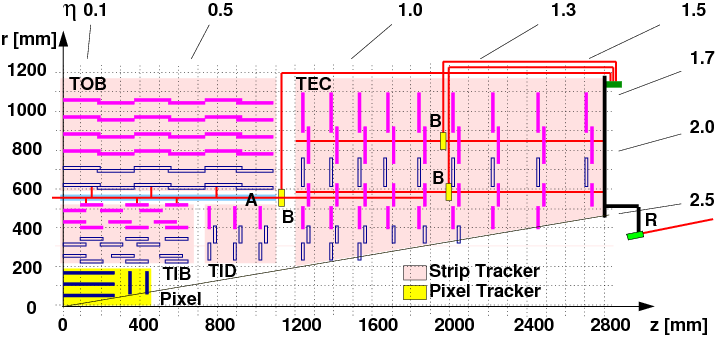
\includegraphics[width=\textwidth]{Images/CMS/TrackerQuadrant.png}
    \caption{A schematic cutaway showing one quadrant of the strip and pixel trackers.}
    \label{fig:StripDiagram}
\end{figure}